% Gate results
\section{Gate results}\label{sec:gates}

\subsection{Setup and SPICE reference}
We evaluate INV, NAND2, NOR2 and AND2/OR2 (NAND2/NOR2 + inverter): 18 input cases, each at the
same \NumCorners{} PVT corners. A corner is one draw of $V_{DD}$, $T$ and the process parameters
(one draw for all NMOS, one for all PMOS); the corners are drawn once (seed \SeedCorners) and
reused by the test circuit. Each of the \NumGateSims{} combinations is simulated as one complete
deck (AND2/OR2 as single decks, not NAND2 + INV added), inputs at exactly $0$ or $V_{DD}$. The
leakage is the supply current $I_{VDD}=-\texttt{i(vvdd)}$; each deck also records the output and
internal nodes ($x$ between series NMOS, $y$ between series PMOS, $n_1$ at the AND2/OR2 first
stage). The output passes the logic check in \GateLogicOk{} rows.

\subsection{From transistor models to gate leakage}
For every (gate, inputs, corner) we (1) take the output and internal node voltages from SPICE, as
the brief prescribes; (2) derive each transistor's $(V_D,V_G,V_S,V_B)$, case, width and corner
parameters from the topology; (3) predict all transistors of all \NumGateSims{} rows in one
batched call; and (4) apply KCL on the VDD net: $I_{VDD}$ is the sum of the currents into all
terminals tied to VDD (PMOS sources and bodies). The same bookkeeping on the input nodes gives
$I_{in}$, the tunnelling current drawn by inputs at logic~1, which the test circuit needs. The
models only saw $V_G\in\{0,V_{DD}\}$, so the AND2/OR2 inverter gate (driven by $n_1$) is snapped to
the nearest rail; the largest snap is \GateSnapMax{}.

\subsection{Why the direct sum failed, and the KCL composition}\label{sec:kcl}
Our first implementation summed the predicted currents directly. With the first models this gave
a median error of \qty{846}{\percent} and \emph{negative} leakage in \qty{77}{\percent} of rows.
The SPICE oracle below showed the bookkeeping was correct, and an attribution traced
\qty{99.7}{\percent} of the error to one term: the channel current of the ON PMOS on the VDD net.

The reason is physical. An ON transistor in a static gate is a closed switch between two nodes at
almost the same voltage: over all gate rows, the \OnVdsCount{} such transistors have median
$|V_{DS}|$ = \OnVdsMedian{} and at most \OnVdsMax. Their channel current is set by the rest of the
gate (typically the OFF device they feed), not by their own minute $V_{DS}$, so predicting it from
$V_{DS}$ is ill-posed: even rounding these voltages to 10 digits changes the SPICE current by
\qty{0.3}{\percent}. More training data near $V_{DS}\approx 0$ fixed the sign but not the
magnitude (60--\qty{100}{\percent} error in our tests).

We therefore treat the channel current of every ON transistor with $|V_{DS}| <$ \KclVdsMax{} as
an unknown. Its predicted $I_G$ and $I_B$ are kept (they have no zero crossing), its drain current
is solved from KCL at the floating nodes (output, $x$, $y$, $n_1$), and $I_S=-(I_D+I_G+I_B)$. All
other transistors keep their model currents. The threshold lies orders of magnitude above the
in-gate ON values and below the smallest genuinely biased ON transistor (\OnBiasedVdsMin, e.g.\
the lower PMOS of NOR2 \texttt{10}), which keeps its model current. Parallel ON transistors (both
PMOS of NAND2 \texttt{00}) leave only their sum determined; we take the minimum-norm
(pseudo-inverse) solution. Any other split adds a current circulating around the parallel loop,
which enters and leaves the VDD net and cannot change $I_{VDD}$; the code checks this for every
pattern. $I_{in}$ is unaffected, since gate currents are never corrected.

\paragraph{SPICE-oracle validation.}
To test the composition independently of the ML models, we simulated every transistor of every
gate row \emph{alone} in ngspice at exactly the terminal voltages the model sees, and fed these
SPICE currents through the same composition. Over all \NumGateSims{} rows this reproduces the
gate SPICE leakage with mean accuracy \OracleMeanAcc{} (median error \OracleMedianErr, p95
\OraclePninetyfiveErr, max \OracleMaxErr). The topology mapping, signs, widths, corner parameters
and the KCL solve are therefore exact well below the ML error, and \emph{all} remaining gate error
comes from the transistor models.

\subsection{Results (D6, D7)}
Over all rows the gate leakage reaches a mean accuracy of \GateMeanAcc{}: median error
\GateMedianErr, p95 \GatePninetyfiveErr, maximum \GateMaxErr, bias \GateBias, and \GateWithinTen{}
of rows within \qty{10}{\percent} of SPICE (Table~\ref{tab:gates}, Figure~\ref{fig:gateparity}).
With the same final models the direct sum reaches only \GateDirectMeanAcc{} (median
\GateDirectMedianErr, p95 \GateDirectPninetyfiveErr): the KCL composition is still essential.

\begin{table}[H]
  \centering
  \small
  \caption{Gate results (D6), KCL composition, \NumCorners{} corners per case: SPICE and ML median
  leakage, bias (median signed error), median and p95 absolute error, mean accuracy. Last row: all
  \NumGateSims{} rows.}
  \label{tab:gates}
  \fittable{% Generated by report/make_numbers.py from results/tables/gate_results.csv. Do not edit.
\begin{tabular}{llrrrrrr}
\toprule
Gate & Inputs & SPICE median (A) & ML median (A) & Bias & Median err. & p95 err. & Mean acc. \\
\midrule
INV & \texttt{0} & \num{1.63e-11} & \num{1.64e-11} & \qty[retain-explicit-plus]{+0.17}{\percent} & \qty{0.98}{\percent} & \qty{2.93}{\percent} & \qty{98.85}{\percent} \\
 & \texttt{1} & \num{5.43e-12} & \num{5.37e-12} & \qty[retain-explicit-plus]{+0.17}{\percent} & \qty{1.34}{\percent} & \qty{4.07}{\percent} & \qty{98.45}{\percent} \\
\midrule
NAND2 & \texttt{00} & \num{1.79e-11} & \num{1.79e-11} & \qty[retain-explicit-plus]{+0.14}{\percent} & \qty{1.16}{\percent} & \qty{3.39}{\percent} & \qty{98.66}{\percent} \\
 & \texttt{01} & \num{1.63e-11} & \num{1.64e-11} & \qty[retain-explicit-plus]{+0.18}{\percent} & \qty{0.98}{\percent} & \qty{2.94}{\percent} & \qty{98.85}{\percent} \\
 & \texttt{10} & \num{1.34e-11} & \num{1.31e-11} & \qty[retain-explicit-plus]{-0.60}{\percent} & \qty{1.62}{\percent} & \qty{8.63}{\percent} & \qty{97.39}{\percent} \\
 & \texttt{11} & \num{1.09e-11} & \num{1.07e-11} & \qty[retain-explicit-plus]{+0.17}{\percent} & \qty{1.34}{\percent} & \qty{4.06}{\percent} & \qty{98.46}{\percent} \\
\midrule
NOR2 & \texttt{00} & \num{3.27e-11} & \num{3.29e-11} & \qty[retain-explicit-plus]{+0.14}{\percent} & \qty{0.96}{\percent} & \qty{2.85}{\percent} & \qty{98.86}{\percent} \\
 & \texttt{01} & \num{1.80e-11} & \num{1.81e-11} & \qty[retain-explicit-plus]{+0.33}{\percent} & \qty{1.09}{\percent} & \qty{3.09}{\percent} & \qty{98.74}{\percent} \\
 & \texttt{10} & \num{2.94e-12} & \num{2.90e-12} & \qty[retain-explicit-plus]{+0.67}{\percent} & \qty{1.95}{\percent} & \qty{7.38}{\percent} & \qty{97.30}{\percent} \\
 & \texttt{11} & \num{4.79e-13} & \num{4.71e-13} & \qty[retain-explicit-plus]{+0.49}{\percent} & \qty{2.33}{\percent} & \qty{7.53}{\percent} & \qty{97.10}{\percent} \\
\midrule
AND2 & \texttt{00} & \num{4.56e-11} & \num{4.55e-11} & \qty[retain-explicit-plus]{+0.18}{\percent} & \qty{0.91}{\percent} & \qty{2.82}{\percent} & \qty{98.89}{\percent} \\
 & \texttt{01} & \num{4.02e-11} & \num{4.05e-11} & \qty[retain-explicit-plus]{+0.01}{\percent} & \qty{0.82}{\percent} & \qty{2.50}{\percent} & \qty{98.99}{\percent} \\
 & \texttt{10} & \num{3.88e-11} & \num{3.84e-11} & \qty[retain-explicit-plus]{-0.41}{\percent} & \qty{1.16}{\percent} & \qty{4.03}{\percent} & \qty{98.59}{\percent} \\
 & \texttt{11} & \num{3.44e-11} & \num{3.45e-11} & \qty[retain-explicit-plus]{+0.28}{\percent} & \qty{0.98}{\percent} & \qty{2.62}{\percent} & \qty{98.89}{\percent} \\
\midrule
OR2 & \texttt{00} & \num{5.91e-11} & \num{5.96e-11} & \qty[retain-explicit-plus]{+0.09}{\percent} & \qty{0.84}{\percent} & \qty{2.42}{\percent} & \qty{99.00}{\percent} \\
 & \texttt{01} & \num{3.49e-11} & \num{3.49e-11} & \qty[retain-explicit-plus]{+0.27}{\percent} & \qty{1.04}{\percent} & \qty{2.85}{\percent} & \qty{98.86}{\percent} \\
 & \texttt{10} & \num{2.23e-11} & \num{2.26e-11} & \qty[retain-explicit-plus]{+0.36}{\percent} & \qty{1.05}{\percent} & \qty{3.21}{\percent} & \qty{98.80}{\percent} \\
 & \texttt{11} & \num{1.80e-11} & \num{1.79e-11} & \qty[retain-explicit-plus]{+0.19}{\percent} & \qty{0.95}{\percent} & \qty{2.80}{\percent} & \qty{98.90}{\percent} \\
\midrule
\textbf{All} &  & \num{2.01e-11} & \num{2.02e-11} & \qty[retain-explicit-plus]{+0.15}{\percent} & \qty{1.13}{\percent} & \qty{4.13}{\percent} & \qty{98.53}{\percent} \\
\bottomrule
\end{tabular}
}
\end{table}

\begin{figure}[H]
  \centering
  \begin{minipage}[t]{0.49\linewidth}
    \centering
    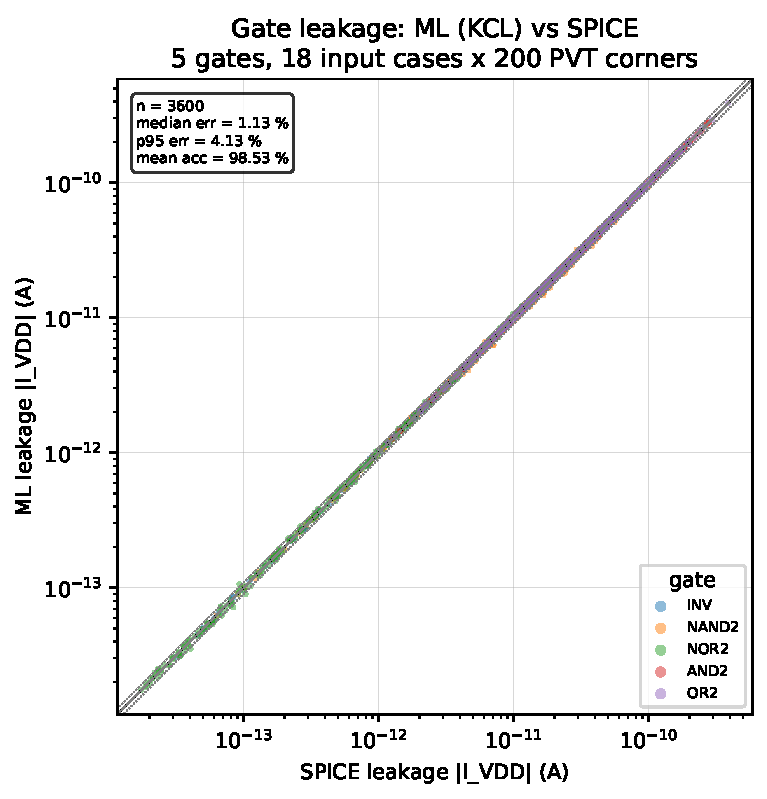
\includegraphics[width=\linewidth]{gate_parity.pdf}
    \caption{Gate parity plot (D7), KCL composition, all \NumGateSims{} rows.}
    \label{fig:gateparity}
  \end{minipage}\hfill
  \begin{minipage}[t]{0.49\linewidth}
    \centering
    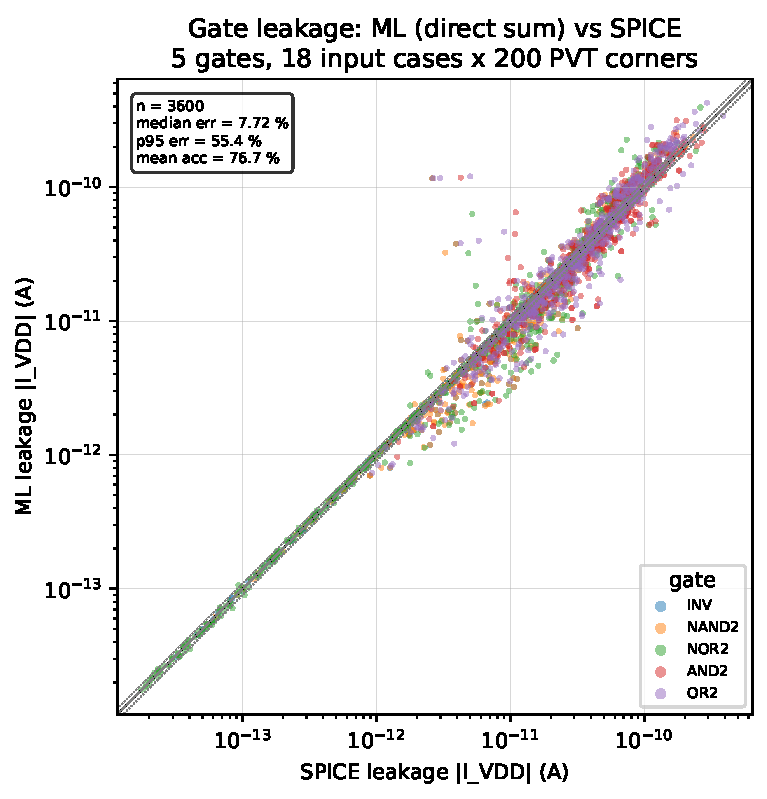
\includegraphics[width=\linewidth]{gate_parity_direct.pdf}
    \caption{Direct sum with the same models. Cases without an ON PMOS on the VDD net agree;
    the others scatter.}
    \label{fig:gateparitydirect}
  \end{minipage}
\end{figure}

\paragraph{Most and least accurate cases.}
The most accurate case is \GateBestCase{} (\GateBestAcc): its leakage is set by OFF transistors at
the full-$V_{DD}$ OFF point that source and drain pinning oversample, while all its ON transistors
are handled by KCL. The least accurate is \GateWorstCase{} (\GateWorstAcc). NAND2 \texttt{10} was the weakest
case for most of the project: its upper NMOS is ON but can only pull $x$ to about a threshold
below $V_{DD}$, so it conducts at a substantial $|V_{DS}|$, is not KCL-corrected, and its predicted
drain current enters the output-node KCL. Before stack pinning, replacing only that current with its SPICE
value raised the case from \qty{94.8}{\percent} to \qty{97.6}{\percent}, which is why we added
stack pinning (Section~\ref{sec:oversampling}); it lifted NAND2 \texttt{10} to \GateNandTenAcc. The
worst individual rows are listed in Table~\ref{tab:gateworst}.

\begin{table}[H]
  \centering
  \small
  \caption{Gate rows with the largest relative error.}
  \label{tab:gateworst}
  \fittable{% Generated by report/make_numbers.py from results/tables/gate_worst_cases.csv. Do not edit.
\begin{tabular}{llrrrrrr}
\toprule
Gate & Inputs & Corner & $T$ (\si{\degreeCelsius}) & $V_{DD}$ (V) & SPICE (A) & ML (A) & Error \\
\midrule
NOR2 & \texttt{10} & 4 & \num{-27.8} & \num{0.980} & \num{8.39e-14} & \num{7.16e-14} & \qty[retain-explicit-plus]{-14.7}{\percent} \\
NOR2 & \texttt{11} & 151 & \num{21.1} & \num{0.852} & \num{9.30e-14} & \num{1.07e-13} & \qty[retain-explicit-plus]{+14.6}{\percent} \\
NOR2 & \texttt{10} & 95 & \num{-26.0} & \num{0.859} & \num{1.03e-13} & \num{8.97e-14} & \qty[retain-explicit-plus]{-13.0}{\percent} \\
NOR2 & \texttt{11} & 195 & \num{9.1} & \num{0.858} & \num{4.03e-14} & \num{3.54e-14} & \qty[retain-explicit-plus]{-12.3}{\percent} \\
NAND2 & \texttt{10} & 25 & \num{53.4} & \num{0.850} & \num{1.66e-11} & \num{1.47e-11} & \qty[retain-explicit-plus]{-11.7}{\percent} \\
NAND2 & \texttt{10} & 186 & \num{69.9} & \num{0.821} & \num{7.08e-12} & \num{6.26e-12} & \qty[retain-explicit-plus]{-11.6}{\percent} \\
NAND2 & \texttt{10} & 119 & \num{99.8} & \num{0.838} & \num{4.61e-12} & \num{4.09e-12} & \qty[retain-explicit-plus]{-11.3}{\percent} \\
NAND2 & \texttt{10} & 184 & \num{123.1} & \num{0.961} & \num{3.82e-11} & \num{3.41e-11} & \qty[retain-explicit-plus]{-10.7}{\percent} \\
NAND2 & \texttt{10} & 64 & \num{64.7} & \num{0.846} & \num{7.02e-12} & \num{6.29e-12} & \qty[retain-explicit-plus]{-10.4}{\percent} \\
NAND2 & \texttt{10} & 145 & \num{43.5} & \num{0.892} & \num{1.87e-11} & \num{1.68e-11} & \qty[retain-explicit-plus]{-10.2}{\percent} \\
NAND2 & \texttt{10} & 65 & \num{92.1} & \num{0.895} & \num{2.39e-11} & \num{2.15e-11} & \qty[retain-explicit-plus]{-10.2}{\percent} \\
NOR2 & \texttt{10} & 87 & \num{-28.5} & \num{0.832} & \num{6.89e-14} & \num{6.22e-14} & \qty[retain-explicit-plus]{-9.7}{\percent} \\
NAND2 & \texttt{10} & 50 & \num{109.0} & \num{0.943} & \num{2.92e-11} & \num{3.19e-11} & \qty[retain-explicit-plus]{+9.3}{\percent} \\
NOR2 & \texttt{11} & 120 & \num{13.4} & \num{0.859} & \num{6.71e-13} & \num{6.10e-13} & \qty[retain-explicit-plus]{-9.1}{\percent} \\
NOR2 & \texttt{10} & 150 & \num{-31.4} & \num{0.976} & \num{1.12e-13} & \num{1.02e-13} & \qty[retain-explicit-plus]{-8.9}{\percent} \\
NOR2 & \texttt{11} & 144 & \num{15.8} & \num{0.921} & \num{2.62e-13} & \num{2.85e-13} & \qty[retain-explicit-plus]{+8.8}{\percent} \\
NAND2 & \texttt{10} & 115 & \num{120.7} & \num{0.851} & \num{2.69e-11} & \num{2.45e-11} & \qty[retain-explicit-plus]{-8.8}{\percent} \\
NOR2 & \texttt{11} & 109 & \num{47.7} & \num{0.838} & \num{4.78e-13} & \num{4.36e-13} & \qty[retain-explicit-plus]{-8.7}{\percent} \\
NAND2 & \texttt{10} & 161 & \num{122.7} & \num{0.853} & \num{1.68e-11} & \num{1.54e-11} & \qty[retain-explicit-plus]{-8.6}{\percent} \\
NAND2 & \texttt{10} & 154 & \num{70.3} & \num{0.824} & \num{4.19e-12} & \num{3.83e-12} & \qty[retain-explicit-plus]{-8.6}{\percent} \\
\bottomrule
\end{tabular}
}
\end{table}

\paragraph{Input current.}
$I_{in}$ is predicted with mean accuracy \GateIinMeanAcc{} (median \GateIinMedianErr, p95
\GateIinPninetyfiveErr, bias \GateIinBias). It is far from negligible: in rows with a high input
it is \GateIinShare{} of $I_{VDD}$ at the median, which matters for the test circuit.

\subsection{How the accuracy developed}\label{sec:history}
Table~\ref{tab:history} summarises our iterations. The large steps came from the composition and
from sampling the right operating points; the model change that mattered was the linear leaves.

\begin{table}[H]
  \centering
  \small
  \caption{Development of the gate-level accuracy (18 cases, \NumCorners{} corners). Rows 1--3
  and 5: earlier runs as recorded; rows 4 and 6: generated.}
  \label{tab:history}
  \begin{tabular}{@{}>{\raggedright\arraybackslash}p{0.52\linewidth}lrr@{}}
    \toprule
    Stage & Composition & Median err. & Mean acc. \\
    \midrule
    1.\ first models, uniform data & direct & \qty{846}{\percent} & -- \\
    2.\ + low-$|V_{DS}|$ ON rows & direct & \qty{14}{\percent} & -- \\
    3.\ + KCL composition & KCL & \qty{7.0}{\percent} & \qty{91.5}{\percent} \\
    4.\ \RowsPerCase{} rows, source and drain pinning, constant leaves & KCL &
        \ConstLeafGateMedianErr & \ConstLeafGateMeanAcc \\
    5.\ + linear-leaf GBDT & KCL & -- & \qty{97.6}{\percent} \\
    6.\ final: + ON stack pinning & KCL & \GateMedianErr & \GateMeanAcc \\
    \bottomrule
  \end{tabular}
\end{table}

\subsection{Generalisation to fresh corners}\label{sec:fresh}
Because the sampling rules were guided by gate errors on the \NumCorners{} evaluation corners, we
repeated the full gate evaluation on \FreshNumCorners{} \emph{new} corners (seed \FreshSeed),
with new SPICE references (logic check \FreshLogicOk) and unchanged models. There is no
degradation (Table~\ref{tab:fresh}): \FreshMeanAcc{} mean accuracy (median \FreshMedianErr, p95
\FreshPninetyfiveErr) against \GateMeanAcc{} on the original corners.

\begin{table}[H]
  \centering
  \small
  \caption{Gate accuracy on the evaluation corners and on \FreshNumCorners{} fresh corners.}
  \label{tab:fresh}
  \fittable{% Generated by report/make_numbers.py from report/analysis/fresh_corners/overall_kcl_direct_orig_vs_fresh.csv. Do not edit.
\begin{tabular}{llrrrrr}
\toprule
Corners & Composition & Median err. & p95 err. & Max err. & Bias & Mean acc. \\
\midrule
original & KCL & \qty{1.82}{\percent} & \qty{6.20}{\percent} & \qty{26.4}{\percent} & \qty[retain-explicit-plus]{+1.04}{\percent} & \qty{97.61}{\percent} \\
 & direct & \qty{7.47}{\percent} & \qty{55.30}{\percent} & \qty{2567.4}{\percent} & \qty[retain-explicit-plus]{-2.02}{\percent} & \qty{79.63}{\percent} \\
\midrule
fresh & KCL & \qty{1.70}{\percent} & \qty{5.93}{\percent} & \qty{29.2}{\percent} & \qty[retain-explicit-plus]{+0.70}{\percent} & \qty{97.69}{\percent} \\
 & direct & \qty{6.92}{\percent} & \qty{52.97}{\percent} & \qty{628.5}{\percent} & \qty[retain-explicit-plus]{-2.19}{\percent} & \qty{83.30}{\percent} \\
\bottomrule
\end{tabular}
}
\end{table}
